Subtracting the background with the rolling ball algorithm unfortunately is still not enough to get a reasonably clean signal of Golgi apparatus from fluorescence imaging, as a lot of background noise will still be present there. In Figure \ref{subfig:vanilla} one can see a fluorescence image preprocessed with a rolling ball algorithm. After turning it into a binary image that can be seen in Figure \ref{subfig:vanilla-mask}, it becomes clear that the images still contains a lot of background low-intensity noise, which was not visible for an eye.
\begin{figure}[htb]
	\centering
	\begin{subfigure}[b]{0.22\textwidth}
		\centering
		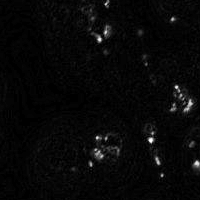
\includegraphics[width=\textwidth]{bilder/preprocessing/crop_golgi_not_full_processed.png}
		\caption{}
		\label{subfig:vanilla}
	\end{subfigure}
	\hfill
	\begin{subfigure}[b]{0.22\textwidth}
		\centering
		
\includegraphics[width=\textwidth]{bilder/preprocessing/crop_golgi_not_full_processed_mask.png}
		\caption{}
		\label{subfig:vanilla-mask}
	\end{subfigure}
	\hfill
	\begin{subfigure}[b]{0.22\textwidth}
		\centering
		
\includegraphics[width=\textwidth]{bilder/preprocessing/crop_golgi_full_processed.png}
		\caption{}
		\label{subfig:clipping}
	\end{subfigure}
	\hfill
	\begin{subfigure}[b]{0.22\textwidth}
		\centering
		
\includegraphics[width=\textwidth]{bilder/preprocessing/crop_golgi_full_processed_mask.png}
		\caption{}
		\label{subfig:clipping-mask}
	\end{subfigure}
	   \caption{(a) Basic preprocessing with automatic background removal algorithm only; (b) binary masked of subfigure (a); (c) Additional clipping of lower intensities after vanilla pre-processing; (d) binary mask of subfigure (c)}
	   \label{fig:pre-processing-golgi}
\end{figure}
In order to get rid of it one could clip lower intensities of the image via image enhancement. In order to do that one can simply clip all the intensities below $90$-th percentile of the image and normalize it afterwards. The result of the clipped image and its mask are illustated in Figure \ref{subfig:clipping}, \ref{subfig:clipping-mask} correspondingly. It contains almost no background noise now. Such additional clipping has improved the results slightly.